\section{Overview of ASIC Testers}
All ASIC testers build upon the same simple interface: 
\begin{enumerate}
\item The user specifies what outputs to expect from their chip in response to what inputs.
\item The system applies the user-specified inputs to the device under test (DUT) and later samples the outputs of the DUT.
\item The machine reports how the sampled outputs compare to the outputs expected by the user.
\end{enumerate}

Below, we dissect and analyze these three steps both abstractly and via the LV500's implementation. Throughout this section, we define some terminology borrowed from the LV500. 

\subsection{Specifying Input Vectors and Output Vectors}
Terminology: 
\begin{itemize}
\item \textbf{Input vector}: An ordered list of 0s and 1s that correspond to some ordering of a subset of the DUT's input pins. 
\item \textbf{Output vector}: An ordered list of \textit{expected} 0s and 1s that correspond to some ordering of a subset of the DUT's output pins. 
\end{itemize}

As ASIC testers are generally not designed with any specific DUT in mind, much more information accompanying input and output vectors must be provided.

\subsubsection{Pin Locations}
Any ASIC tester will define "pin locations" that are associated with some kind of socket used to connect a DUT to the tester. Obviously, mapping pins on a DUT to pin locations on an ASIC tester varies per tester. The key idea to keep in mind is that the user does not have to inform the tester of every input and output signal on the DUT. Only the pins on the DUT that the user wishes to test must be mapped to the tester's pin locations. Depending on the tester, any unspecified DUT pins may be left floating or pulled high/low with a resistor.

\subsubsection{Inputs and Outputs}
\begin{flushleft}
Terminology: 
\begin{itemize}
\item \textbf{Pin direction}: A designator that specifies whether a DUT pin is an input or output.
\item \textbf{Template}: A bit vector that maps DUT pins to pin directions.
\end{itemize}
\end{flushleft}

In addition to providing the locations of the DUT pins to test, the user must specify the direction of these types of pins using templates. Every input and output vector is associated with some template. For bidirectional pins, different templates can be applied at different phases throughout a test. One template may designate a signal X as an input while a different template may designate that same signal X as an output. 

Thus far, we have described (abstractly) how to tell an ASIC tester about the pins on a DUT that we wish to test, which of those pins are inputs/outputs, and the signals that we expect to see in response to the signals that we wish to apply to the input pins. We must answer two other questions for the ASIC tester: 

\begin{enumerate}
\item When should input signals be applied to the DUT's input pins, and when should signals from the DUT's output pins be sampled?
\item After we apply the input signals to the DUT, what should we do with the input signals before and after the output pins are sampled?
\end{enumerate}

\subsection{Test Cycles}
One thing we must specify is when input signals to the DUT should be applied and when output signals of the DUT should be sampled.

\begin{flushleft} 
Terminology:  
\begin{itemize}
\item \textbf{Test cycle}: A window of time wherein an input vector is forced upon the DUT and the output signals of the DUT are (later) sampled.
\item \textbf{Test cycle length}: The length (in time) of a test cycle.
\item \textbf{Test cycle delay}: The amount of time between the beginning of the test cycle and when an input vector should be forced upon the DUT.
\item \textbf{Test cycle width}: The amount of time between when an input vector should be forced upon the DUT and when the output signals of the DUT should be sampled.
\item \textbf{Test}: The execution of all input vectors specified by the user.
\end{itemize}
\end{flushleft}

Figure \ref{fig:singleTestCycle} below illustrates how a test cycle can be thought of as just a configurable pulse (though test cycles don't necessarily have to be implemented as an actual pulse). It is important to note that the test cycle itself is NOT sent to the DUT. Test cycles use two edges (a rising edge and falling edge) to signify when to force inputs and sample outputs, respectively.

\begin{flushleft}
Terminology: 
\begin{itemize}
\item \textbf{Leading edge}: A rising edge that corresponds to a test cycle's delay.
\item \textbf{Trailing edge}: A falling edge that corresponds to a test cycle's width.
\end{itemize}
\end{flushleft}

To get a sense of how test cycles are used, consider Figure \ref{fig:ANDGateTestCycle} below. Assume the following setup as the context of this figure: 
\begin{itemize}
\item Our DUT contains three pins mapping to a two-input AND gate that we wish to test.
\item We have informed the ASIC tester of where these three pins are located, which two of the three pins are inputs, and which of the three pins is the output. (We have also named the input pins A and B and the output pin Y for convenience.)
\item We have specified two input vectors: {A = 1, B = 1} and {A = 0, B = 0}, along with two corresponding output vectors: {Y = 1} and {Y = 0}.
\item We specified a test cycle length of 100 ns, a test cycle delay of 20 ns, and a test cycle width of 50 ns.
\end{itemize}

\begin{figure}
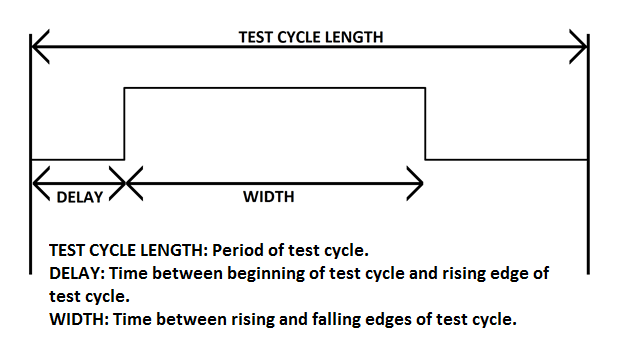
\includegraphics[width=1.0\textwidth]{test_cycle1.png}
\caption{A single test cycle.}
\label{fig:singleTestCycle}
\end{figure}

\begin{figure}
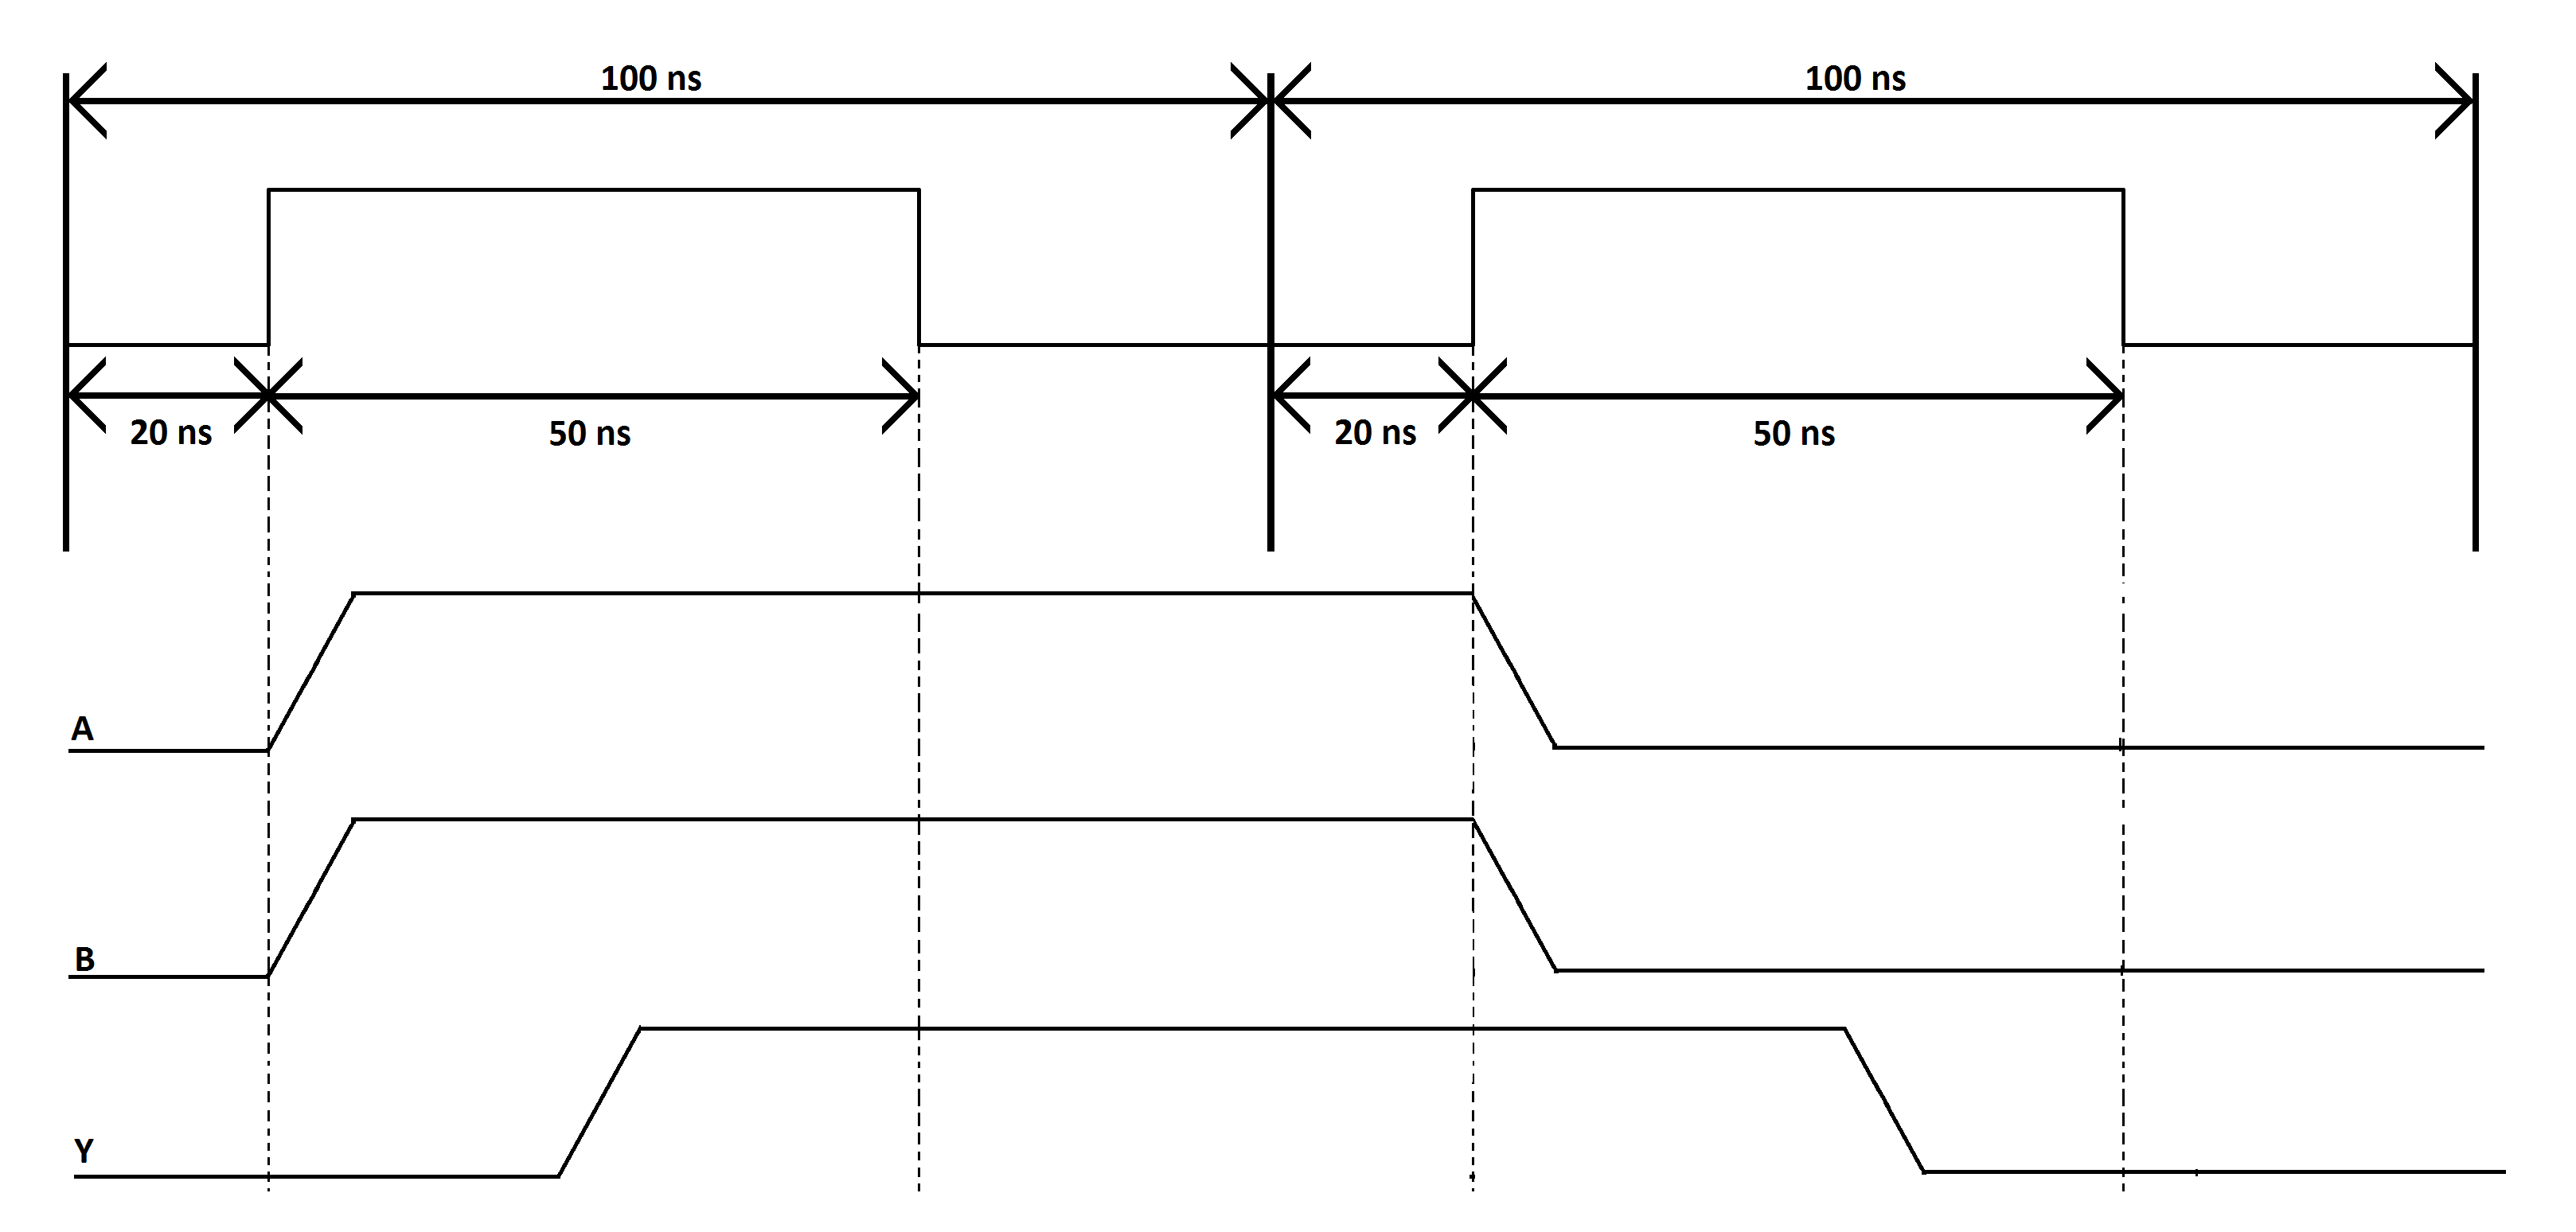
\includegraphics[width=1.0\textwidth]{test_cycle3.png}
\caption{Testing an AND gate with a test cycle configured to have a length of 100 ns, a delay of 20 ns, and a width of 50 ns. Two input vectors (and thus two cycles) are applied to the DUT.}
\label{fig:ANDGateTestCycle}
\end{figure}

\subsection{Force Formats}
Note that in Figure \ref{fig:ANDGateTestCycle}, the inputs A and B latch onto whatever value they are assigned at every leading edge. It may be desirable to have A and B behave differently, however. For instance, we may want A and B to latch onto whatever value they are assigned at every leading edge, but return to 0 at every trailing edge. For versatile testing, an ASIC tester must also provide (what the LV500 calls) force formats to be associated with every input pin.

\begin{flushleft}
Terminology: 
\begin{itemize}
\item \textbf{Force format}: A specification for how an input signal should behave during a test cycle. 
\end{itemize}
\end{flushleft}

\textit{An aside}: The LV500 uses the term "force" to refer to applying inputs to DUT pins, hence the phrase "force format".

The LV500 defines five natural force-formats: 
\begin{itemize}
\item \textbf{R0}: Inputs latch onto their assigned values on leading edges, but return to 0 on trailing edges. (Return to zero.)
\item \textbf{R1}: Inputs latch onto their assigned values on leading edges, but return to 1 on trailing edges. (Return to one.)
\item \textbf{DNRZ L}: Inputs latch onto their assigned values on leading edges. (Delayed non-return-to-zero, leading edge.)
\item \textbf{DNRZ T}: Inputs latch onto their assigned values on trailing edges. (Delayed non-return-to-zero, trailing edge.)
\item \textbf{R INH}: Inputs latch onto their assigned values on leading edges, but return to high-Z on trailing edges. (Return to inhibited.)
\end{itemize}

Figure \ref{fig:ANDGateTestCycleFF} below is the same setup as Figure \ref{fig:ANDGateTestCycle}, but with the R0 force-format used for A and B (as opposed to the DNRZ L force-format). Note that A and B do not have to be assigned the same force-format! Any ASIC tester should allow every individual pin to be associated with its own force-format. In this case, there is nothing invalid about input A being associated force-format R0 and input B being associated force-format R1, for instance.

\begin{figure}
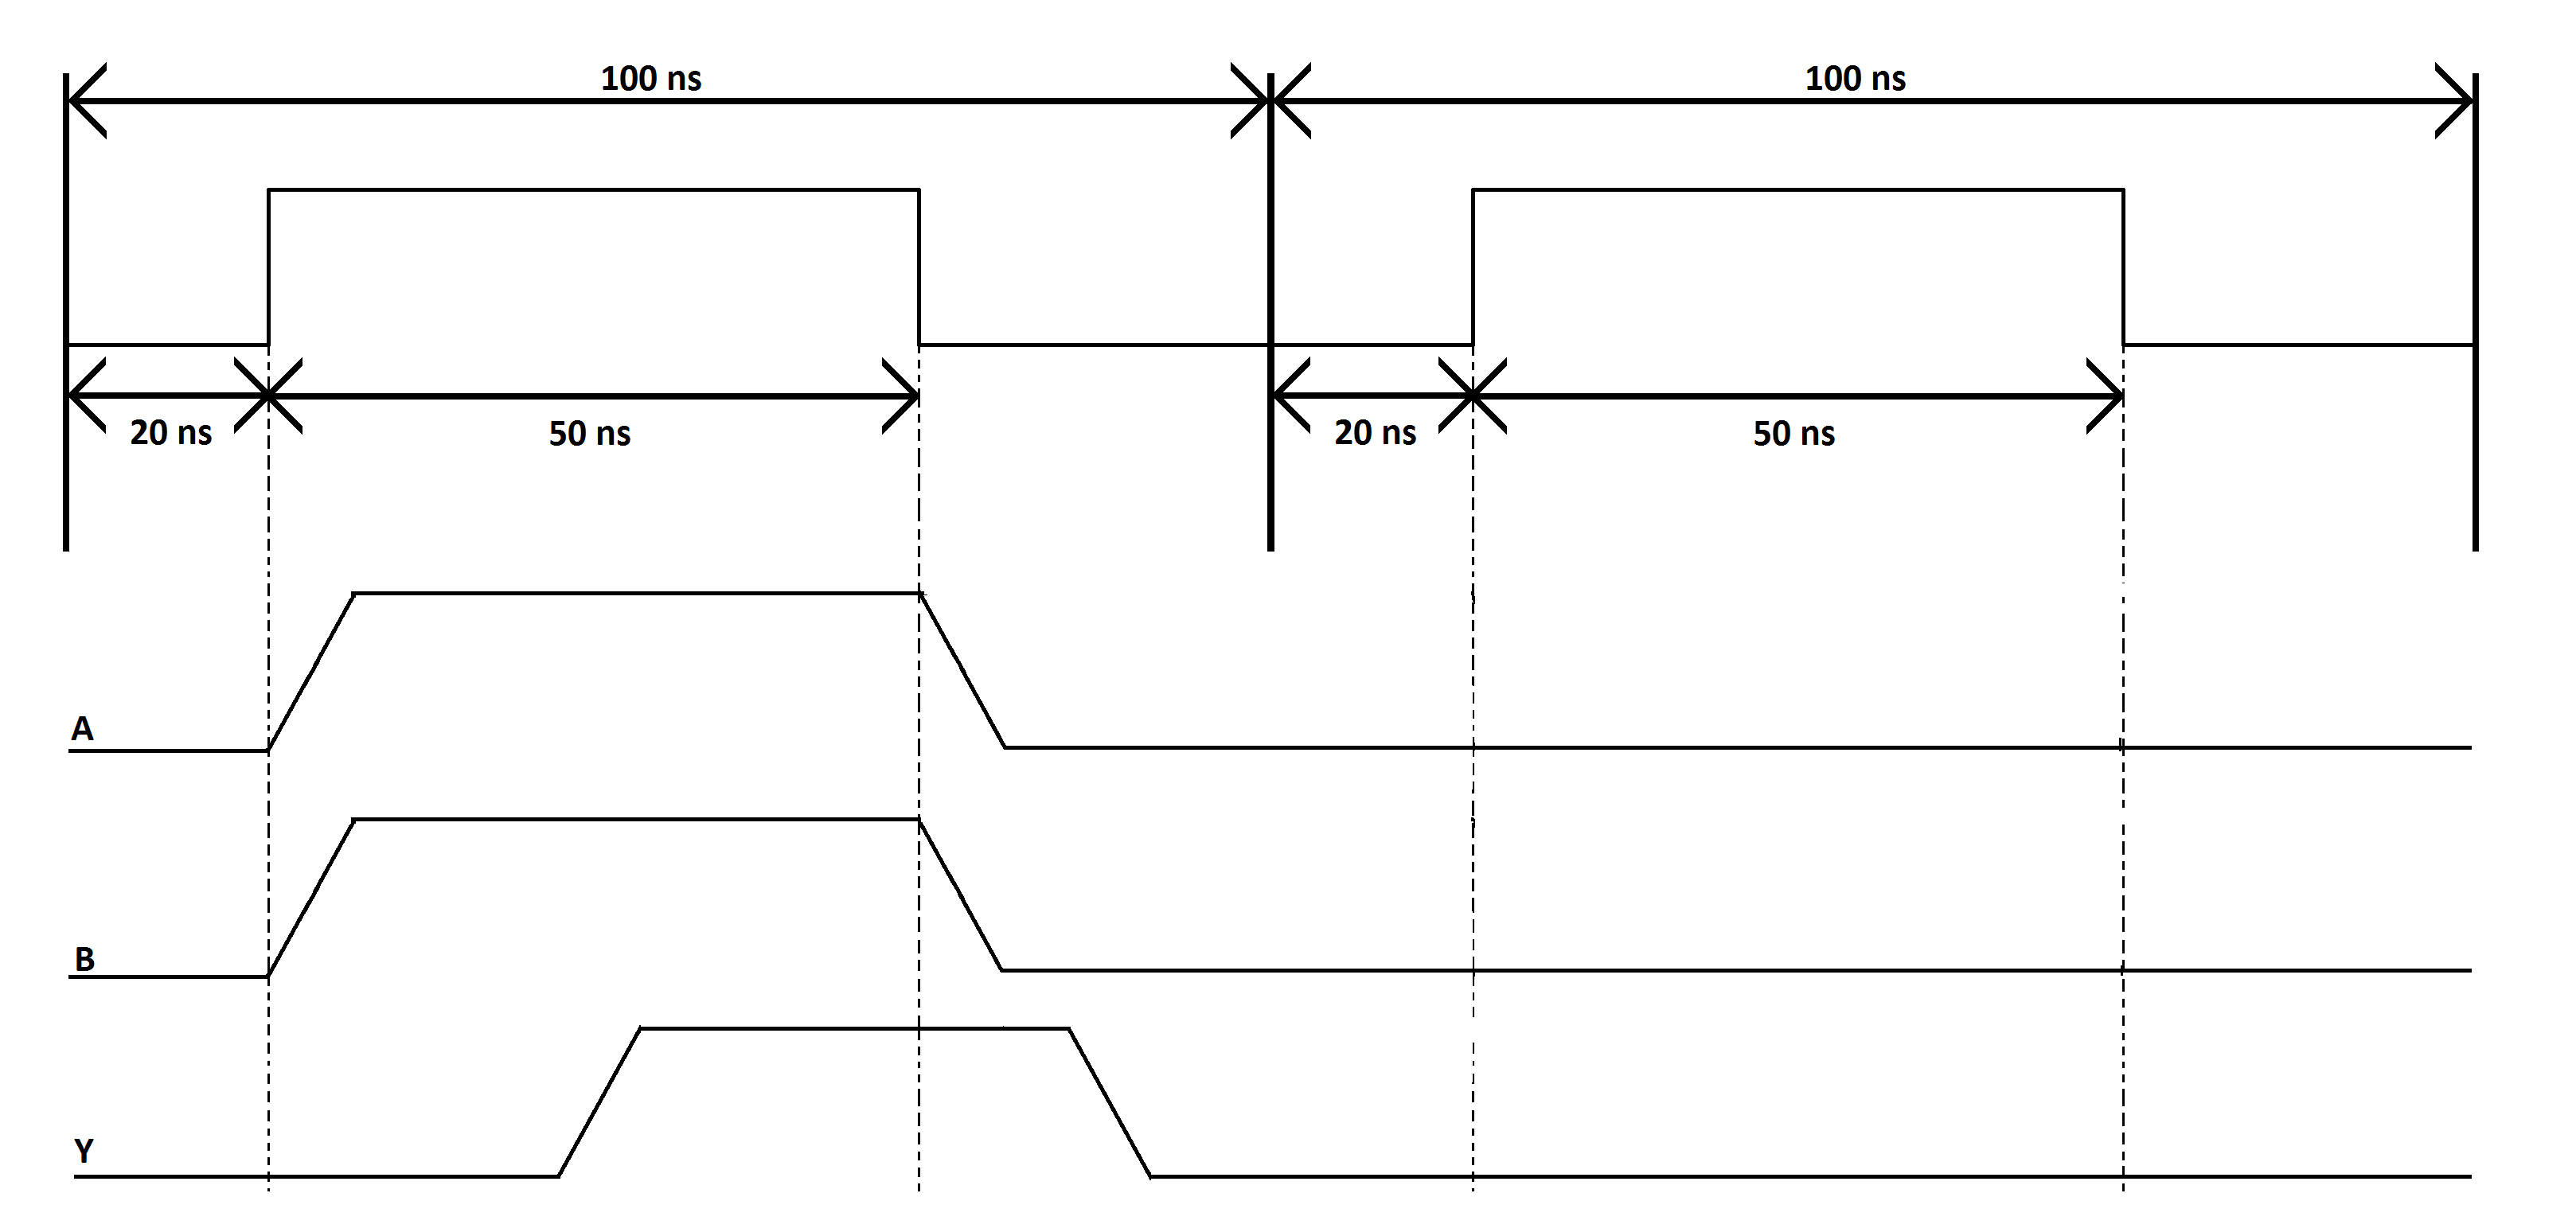
\includegraphics[width=1.0\textwidth]{test_cycle4.png}
\caption{The same configuration as Figure \ref{fig:ANDGateTestCycle} but with a different force format for the inputs.}
\label{fig:ANDGateTestCycleFF}
\end{figure}

\subsection{Combinational Circuits vs. Sequential Circuits}
As shown with Figures \ref{fig:ANDGateTestCycle} and \ref{fig:ANDGateTestCycleFF}, testing a combinational circuit is fairly straightforward. On the other hand, testing a sequential circuit requires more functionality from an ASIC tester. We certainly don't want to transition the clock signal at the same time as the inputs -- otherwise, we may violate the setup times of registers within the DUT. A solution to this problem is to allow every pin to be associated with a test cycle. Consider Figure \ref{fig:DFFTestCycles} below, which demonstrates testing a D Flip-Flop (DFF). We associate the D input to the DFF with the uppermost test cycle and the CLK input to the DFF with the lowermost test cycle. As seen in the figure, we allow D 20 ns to settle on the input to the DFF before we transition the clock. Note that the output of the DFF, Q, needs to be associated with one of the two test cycles in the figure. Whichever test cycle Q is associated with, we sample Q on the trailing edge of the cycle.

\begin{figure}
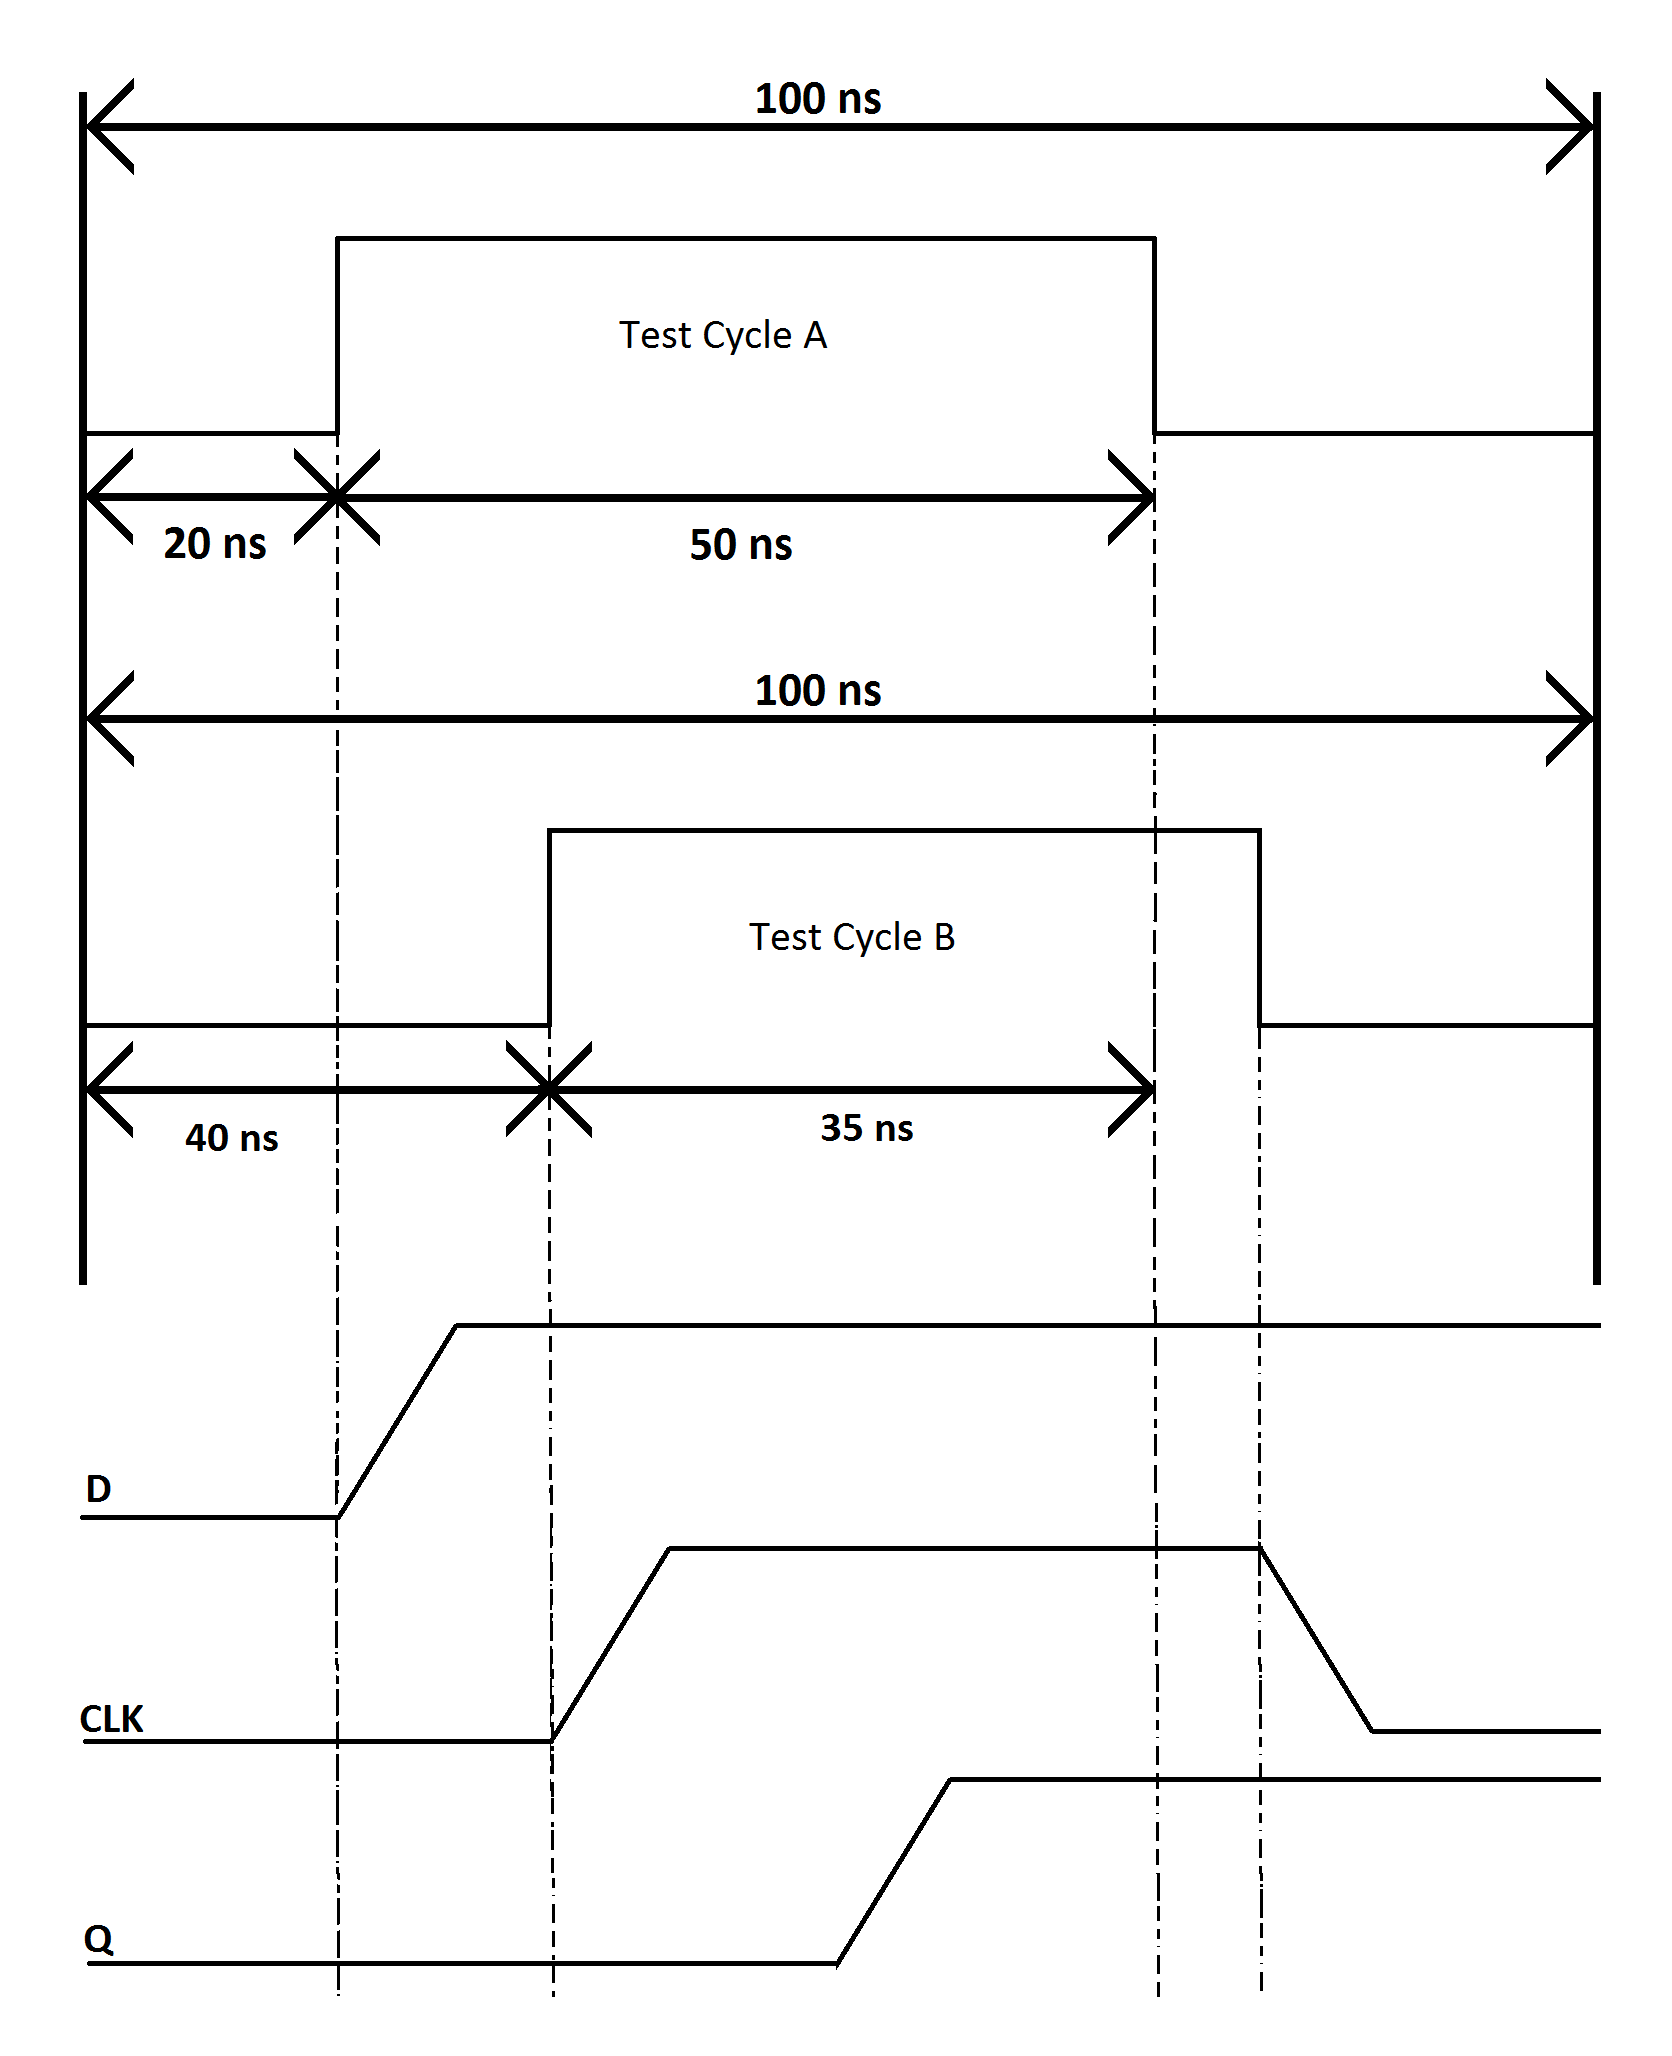
\includegraphics[width=1.0\textwidth]{test_cycle2.png}
\caption{Testing a D Flip-Flop.}
\label{fig:DFFTestCycles}
\end{figure}

\subsection{Electrical and Dynamic Configurations}
A DUT may require a variety of different VDDs -- 5V, 3.3V, 1.8V, etc., so an ASIC tester needs to provide different VDDs for different chips. More interesting, however, is how a DUT may respond to unideal high and low voltage values. For instance, if we know that logic low values may range between 0V and 0.5V and that logic high values may range between 4.2V and 5V, it'd be interesting to know how a DUT will respond to these kinds of voltage values.

Additionally, it may be worth knowing how fast our DUT is. Consider Figure \ref{fig:DFFTestCycles}, where we test a DFF. One way to estimate the setup time of the DFF would be to gradually bring the two leading edges closer to each other until the Q output fails to meet our expectations.

\begin{flushleft}
Terminology: 
\begin{itemize}
\item \textbf{Schmooing}: Repeating a test some number of times, with just one electrical or timing characteristic differing between tests.
\end{itemize}
\end{flushleft}

Consider Figure \ref{fig:ANDGateTestCycleFF}, where we perform a simple test of an AND gate using two input vectors. An example of schmooing would be repeating the entire test, but with the VDD for the input signals starting at 5V for the first test and dropping by 0.2V on each subsequent test until VDD reaches 4.2V. (So, a total of five tests, where each test consists of two test cycles.) Another example, with Figure \ref{fig:DFFTestCycles}, would be to increase the delay of the uppermost test cycle by 1 ns on each subsequent test up to 40 ns. (So, a total of 20 tests.)

Even better, the LV500 allows users to generate plots of the percentage of output vectors that pass in comparison to the one or two electrical/timing characteristics schmooed. 

\subsection{Further Reading}
Refer to \href{https://view.officeapps.live.com/op/view.aspx?src=http://www.ece.utah.edu/~kstevens/6712/tester.ppt}{these slides} for more information on how the LV500 works.

\newpage
